\documentclass[a4paper, 10pt, ]{article}

\usepackage[slovak]{babel}





\usepackage[utf8]{inputenc}
\usepackage[T1]{fontenc}

\usepackage[left=4cm,
			right=4cm,
            % left=2.5cm,
			% right=5.5cm,
			top=2.1cm,
			bottom=2.6cm,
			footskip=7.5mm,
			% twoside,
			marginparwidth=3.0cm,
			%showframe,
			]{geometry}

\usepackage{graphicx}
\usepackage[dvipsnames]{xcolor}
% https://en.wikibooks.org/wiki/LaTeX/Colors


% ------------------------------

\usepackage{lmodern}

\usepackage[tt={oldstyle=false,proportional=true,monowidth}]{cfr-lm}

% ------------------------------

\usepackage{amsmath}
\usepackage{amssymb}
\usepackage{amsthm}

\usepackage{booktabs}
\usepackage{multirow}
\usepackage{array}
\usepackage{dcolumn}


\usepackage[singlelinecheck=true]{subfig}


% ------------------------------


\def\naT{\mathsf{T}}

\hyphenpenalty=6000
\tolerance=1000




% ------------------------------


\makeatletter

	\def\@seccntformat#1{\protect\makebox[0pt][r]{\csname the#1\endcsname\hspace{4mm}}}

	\def\cleardoublepage{\clearpage\if@twoside \ifodd\c@page\else
	\hbox{}
	\vspace*{\fill}
	\begin{center}
	\phantom{}
	\end{center}
	\vspace{\fill}
	\thispagestyle{empty}
	\newpage
	\if@twocolumn\hbox{}\newpage\fi\fi\fi}

	\newcommand\figcaption{\def\@captype{figure}\caption}
	\newcommand\tabcaption{\def\@captype{table}\caption}

\makeatother


% ------------------------------




\usepackage{fancyhdr}
\fancypagestyle{plain}{%
\fancyhf{} % clear all header and footer fields
\fancyfoot[C]{\sffamily {\bfseries \thepage}\ | {\scriptsize\oznacenieCasti}}
\renewcommand{\headrulewidth}{0pt}
\renewcommand{\footrulewidth}{0pt}}
\pagestyle{plain}


% ------------------------------


\usepackage{titlesec}
\titleformat{\paragraph}[hang]{\sffamily  \bfseries}{}{0pt}{}
\titlespacing*{\paragraph}{0mm}{3mm}{1mm}
\titlespacing*{\subparagraph}{0mm}{3mm}{1mm}

\titleformat*{\section}{\sffamily\Large\bfseries}
\titleformat*{\subsection}{\sffamily\large\bfseries}
\titleformat*{\subsubsection}{\sffamily\normalsize\bfseries}






% ------------------------------

\PassOptionsToPackage{hyphens}{url}
\usepackage[pdfauthor={},
			pdftitle={},
			pdfsubject={},
			pdfkeywords={},
			% hidelinks,
			colorlinks=false,
			breaklinks,
			]{hyperref}


% ------------------------------


\graphicspath{%
{../fig_standalone/}%
{../../PY/fig/}%
{../../PY/jupynotex/fig/}%
{../../ML/fig/}%
{./fig/}%
}



% ------------------------------

\usepackage{enumitem}

\usepackage{lettrine}

% ------------------------------


\usepackage{microtype}


% ------------------------------

\usepackage[titles]{tocloft}

\setlength{\cftsecindent}{-12mm}
\setlength{\cftsecnumwidth}{12mm}
\renewcommand{\cftsecpresnum}{\hfill}
\renewcommand{\cftsecaftersnum}{\hspace{4mm}}

\setlength{\cftsubsecindent}{-12mm}
\setlength{\cftsubsecnumwidth}{16mm} % 12 + 4
\renewcommand{\cftsubsecpresnum}{\hfill}
\renewcommand{\cftsubsecaftersnum}{\hspace{8mm}} % 4 + 4 mm

\setlength{\cftsubsubsecindent}{-12mm}
\setlength{\cftsubsubsecnumwidth}{20mm} % 12 + 4 + 4
\renewcommand{\cftsubsubsecpresnum}{\hfill}
\renewcommand{\cftsubsubsecaftersnum}{\hspace{12mm}} % 4 + 4 + 4 mm

\renewcommand{\cftsecpagefont}{\lstyle \bfseries}
\renewcommand{\cftsubsecpagefont}{\lstyle}
\renewcommand{\cftsubsubsecpagefont}{\lstyle}



\setlength{\cftparaindent}{-16mm}
\setlength{\cftparanumwidth}{28mm} % 16 + 4 + 4 + 4
\renewcommand{\cftparapresnum}{\hfill}
\renewcommand{\cftparaaftersnum}{\hspace{16mm}} % 4 + 4 + 4 + 4 mm








% ------------------------------

\usepackage{listings}



\renewcommand{\lstlistingname}{Výpis kódu}
\renewcommand{\lstlistlistingname}{Výpisy kódu}




%New colors defined below
\definecolor{codegreen}{rgb}{0,0.6,0}
\definecolor{codegray}{rgb}{0.5,0.5,0.5}
\definecolor{codepurple}{rgb}{0.58,0,0.82}
\definecolor{backcolour}{rgb}{0.95,0.95,0.95}

%Code listing style named "mystyle"
\lstdefinestyle{mystyle}{
  backgroundcolor=\color{backcolour},
  commentstyle=\fontfamily{lmtt}\fontsize{8.5pt}{8.75pt}\selectfont\color{codegreen},
  keywordstyle=\fontfamily{lmtt}\fontsize{8.5pt}{8.75pt}\selectfont\bfseries\color{Blue},
  stringstyle=\fontfamily{lmtt}\fontsize{8.5pt}{8.75pt}\selectfont\color{codepurple},
  basicstyle=\fontfamily{lmtt}\fontsize{8.5pt}{8.75pt}\selectfont,
  breakatwhitespace=false,
  breaklines=true,
  captionpos=t,
  keepspaces=true,
  numbers=left,
  numbersep=4mm,
  numberstyle=\fontfamily{lmtt}\fontsize{8.5pt}{8.75pt}\selectfont\color{lightgray},
  showspaces=false,
  showstringspaces=false,
  showtabs=false,
  tabsize=2,
  % xleftmargin=10pt,
  framesep=10pt,
  language=Python,
  escapechar=|,
}


\lstset{
    inputencoding=utf8,
    extendedchars=true,
    literate=%
    {á}{{\'a}}1
    {č}{{\v{c}}}1
    {ď}{{\v{d}}}1
    {é}{{\'e}}1
    {ě}{{\v{e}}}1
    {í}{{\'i}}1
    {ň}{{\v{n}}}1
    {ó}{{\'o}}1
    {ř}{{\v{r}}}1
    {š}{{\v{s}}}1
    {ť}{{\v{t}}}1
    {ú}{{\'u}}1
    {ů}{{\r{u}}}1
    {ý}{{\'y}}1
    {ž}{{\v{z}}}1
    {Á}{{\'A}}1
    {Č}{{\v{C}}}1
    {Ď}{{\v{D}}}1
    {É}{{\'E}}1
    {Ě}{{\v{E}}}1
    {Í}{{\'I}}1
    {Ň}{{\v{N}}}1
    {Ó}{{\'O}}1
    {Ř}{{\v{R}}}1
    {Š}{{\v{S}}}1
    {Ť}{{\v{T}}}1
    {Ú}{{\'U}}1
    {Ů}{{\r{U}}}1
    {Ý}{{\'Y}}1
    {Ž}{{\v{Z}}}1
    {ô}{{\^{o}}}1
}


% ------------------------------


\usepackage{caption}

\DeclareCaptionFormat{odsadene}{\protect\makebox[0pt][r]{#1#2\hspace{4mm}}#3\par}
\DeclareCaptionLabelSeparator{lendvojbodka}{:}
% \DeclareCaptionFont{lightgray}{\color{lightgray}}
\DeclareCaptionFont{lightgray}{\fontfamily{lmtt}\fontsize{8.5pt}{8.75pt}\selectfont\color{lightgray}}

\captionsetup[lstlisting]{format=odsadene, labelsep=lendvojbodka, justification=raggedright, singlelinecheck=false, labelfont={sf, lightgray},}


% ------------------------------





% ------------------------------

\usepackage[backend=biber,
            style=numeric,
            sorting=none,
            ]{biblatex}
\DeclareSourcemap{
    \maps[datatype=bibtex]{
        \map{
        \step[fieldset=note, null]
        }
        \map{
        \step[fieldset=file, null]
        }        
        % \map{
        % \step[fieldset=url, null]        
        % }
        \map{
        \step[fieldset=eprint, null]
        }
    }
}


\addbibresource{E:/_CurrentContent/01_work_repo/bibLaTeXDB/bibLaTeXDB.bib} % nonpublic data





\def\oznacenieCasti{MRS02 - ZS2025}


\usepackage{longtable}




\begin{document}


\lstset{%
style=mystyle,
rangebeginprefix=\#\#\#\ cellB\ ,%
rangebeginsuffix=\ \#\#\#,%
rangeendprefix=\#\#\#\ cellE\ ,%
rangeendsuffix=\ \#\#\#,%
includerangemarker=false,
}





\fontsize{12pt}{22pt}\selectfont

\centerline{\textsf{Modelovanie a riadenie systémov} \hfill \textsf{\oznacenieCasti}}

\fontsize{18pt}{22pt}\selectfont





\begin{flushleft}
	\textbf{\textsf{Prednáška úvodná}}
\end{flushleft}






\normalsize

\bigskip

{\hypersetup{hidelinks}

\tableofcontents

}

\bigskip

\vspace{18pt}



\noindent
\lettrine[lines=3, nindent=0pt]{C}{ieľom} tohto textu je najmä vytvoriť akýsi úvodný zoznam pojmov, s ktorými potrebuje čitateľ pracovať pri štúdiu v oblasti kybernetiky, robotiky, teórie riadenia a tak podobne. Vo všeobecnosti ide o~značne široké pojmy avšak v~tomto texte je možné vidieť ako sa s nimi pracuje z hľadiska technickej kybernetiky, z~hľadiska (technickej) teórie systémov, z~hľadiska automatizácie a~z~hľadiska riadiacich systémov.








\section{Predmet Modelovanie a riadenie systémov}

Predmet \emph{Modelovanie a riadenie systémov} možno rozdeliť na dve hlavné časti: modelovanie systémov a riadenie systémov. Pre obe časti platí, že ide o~prvotný súbor informácii pre čitateľa, ktorého cieľom je štúdium kybernetiky, robotiky, prípadne ďalej teórie riadenia, identifikácie systémov atď. (veľmi rozsiahle možnosti).

\begin{center}

    \vbox{%
        \makebox[\textwidth][c]{%
        \input{../fig_standalone/schURO_vseob.pdf_tex}
        }
        \figcaption{Uzavretý regulačný obvod. Časť predmetu Modelovanie a riadenie systémov sa týka riadeného systému (jeho matematické modelovanie) a časť predmetu sa týka riadiaceho systému.}
    }
	\label{schURO_vseob}

\end{center}


\paragraph{Matematika}

Pre prácu v tomto predmete (alebo v týchto oblastiach) je prakticky nevyhnutné využívať isté nástroje, tu sa tým myslia znalosti a praktické zručnosti najmä (ale nie len) z matematiky - diferenciálny a integrálny počet, práca s maticami a algebra. Predmet nie je zameraný na tieto oblasti. Predmet ich využíva. Je veľmi výhodné ak sa študent s~využívaním týchto nástrojov stretol v minulosti, ale nie je to nevyhnutné. Všetko potrebné bude obsiahnuté v predmete, avšak často len v minimálnej miere s~tým, že čitateľ by mal mať jasno v tom akým smerom vo využívaní týchto nástrojov (matematiky napríklad) by sa mal vydať.


\paragraph{Softvér a výpočtové nástroje}

Veľmi súvisiacou sadov nástrojov, ktoré je tu potrebné využívať, je výpočtový softvér, typu MATLAB, GNU Octave, knižnice NumPy pre Python a podobné knižnice pre iné skriptovacie jazyky ako Julia, R a podobne. Rovnako však platí, že v rámci predmetu bude poskytnuté všetko potrebné pre úspešnú prácu a pre ďalšie rozširovanie si vedomostí, skúseností a zručností (v jednom predmete samozrejme nie je možné obsiahnuť všetko).

\bigskip

Hlavným cieľom predmetu je teda vytvoriť priestor pre prvý kontakt s pojmami diskutovanými nižšie avšak nie vo všeobecnosti ale z hľadiska kybernetiky, teórie riadenia, automatizácie a tak podobne.





\section{Kybernetika}

\subsection{Kybernetika a matematika}

Z istého hľadiska na históriu matematiky ako takej je možné usúdiť, že Kybernetika je relatívne mladým odborom matematiky, ktorý vznikol približne v polovici 20.~storočia~\cite{Mares2008}.

Kybernetika je veda. Pri prvom pohľade sa jednoznačne javí ako technická veda. Obzvlášť ak uvážime iné odbory, ktoré vzišli z Kybernetiky ako napríklad informatika, robotika a podobne. Neúplným by bolo konštatovanie, že v Kybernetike ide len o~technické úlohy a problémy, o~stroje a ich riadenie, o~počítače a o~riadiace systémy vo všeobecnosti. Sú to však práve počítače, automatizované stroje a technické aplkikácie vo všeobecnosti, ktoré umožňujú prepájať teóriu (matematickú) s každodenným životom. Často je to práve Kybernetika, ktorá nachádza cestu od matematických teórií, vrátane tých najabstraktnejších, až po konkrétne aplikácie v reálnom svete. 

Kybernetiku je možné napríklad deliť na teoretickú a technickú. Rovnako ako napríklad informatiku. Dôležitým je brať na zreteľ, že sa tým myslia prepojenia na iné vedy, technické odbory a podobne. Výsledky teoretickej Kybernetiky môžu stavať na výsledkoch a nástrojoch z matematiky a~iných oblastí teoretického charakteru a~výsledkami technickej Kybernetiky možno nazvať uplatnenie abstraktnej teórie pri konkrétnych technických problémoch.

Kybernetika a to, čo z nej vzniká, nie je vyústením matematiky, ale jedným z~mostov medzi matematikou a inými odbormi (vedeckými aj praktickými). Matematika sa vyvíja ďalej a bude sa vyvíjať ďalej. Kybernetika vytvára cestu, po ktorej sa matematika dostáva k ľuďom do každodenného života. Veľké na nej je, že tým zmenila a mení svet ako sotva iná veda pred ňou~\cite{Mares2008}.



\subsection{História Kybernetiky}

Vznik Kybernetiky je daný tým, že najmä v jej začiatkoch ide o súbeh vedných odborov, ktoré sa v istých bodoch stretávajú, prelínajú a ovplyvňujú. Dajú sa rozdeliť na skupiny:
\begin{itemize}[leftmargin=0pt, labelsep=3mm, itemsep=0pt]
    \item vedné odbory o riadení systémov a rozhodovaní,
    \item vedné odbory o spracovaní a prenose informácií
    \item počítačové vedy v užšom zmysle automatov a algoritmov.
\end{itemize}


Klasickou definíciou Kybernetiky je definícia vyplývajúca z diela Norberta Wienera z~roku 1948: \emph{Kybernetika je veda riadení a~komunikácii v živých organizmoch, ľudskej spoločnosti a~v~strojoch}~\cite{Wiener2019}.

Práve Norbert Wiener je považovaný za prvého autora, ktorý vídí vyššie uvedené odbory vedy ako zmysluplný samostatný celok, ako samostatnú vedu a pomenúva ju kybernetika. Z jeho diela tiež plynie, že pre Kybernetiku nie je podstatná hmota (a energia), ktorá do skúmaného procesu, deja alebo objektu vstupuje (a vystupuje). Podstatná je štruktúra, ktorú v nich tvorí, a zákonitosti, ktorými sa táto štruktúra riadi.



\subsubsection{Pred pojmom kybernetika}

Myšlienka o tom, že by mohla existovať podobnosť medzi mechanickým zariadením a~činnosťou živého organizmu, alebo dokonca ľudského mozgu existovala už relatívne dávno~\cite{Mares2008}.

\begin{itemize}[leftmargin=0pt, labelsep=3mm, itemsep=0pt]
    \item cca 230 pred n. l., Alexandria, grék Ktesibios -- vodné hodiny, ktoré „sami regulovali“ svoj chod (využitie princípu spätnej väzby)
    \item cca 80 pred n. l., Grécko -- mechanický kalendár schopný predikovať zatmenia Slnka, Mesiaca možno aj pohyb niektorých planét (stroj schopný relatívne náročných výpočtov).
    \item 11. storočie, Čína, astronóm a vynálezca Su Song -- konštruoval rôzne mechanizmy a~nezávisle na európanoch objavil princíp spätnej väzby. \newline Mimochodom, kvalitatívne išlo o technické riešenia konkrétneho problému a to vlastne až po obdobie Wattovho regulátora parného stroja (r. 1788). Nešlo o riešenia založené na matematike, na analýze, na teórii. Kybernetickou na tom je samotná myšlienka, že neživý stroj by mohol sám seba regulovať, riadiť.
\end{itemize}

\noindent
Toľko pre ilustráciu, obdobných rôznych vynálezov by sme v histórií ľudstva našli samozrejme oveľa viac.

\begin{itemize}[leftmargin=0pt, labelsep=3mm, itemsep=0pt]
    \item V rokoch 1898 až 1924 vznikajú články a spisy Jaroslava Janoviča Grdinu, ktorý sa narodil v Plzni ako Jaroslav Hrdina, s rodičmi sa pre prácu presťahovali do Ruska a~on sa nakoniec usadil na Ukrajine. Bol banským inžinierom a vysokoškolským učiteľom \newline Skúmal aj ľudské a živočíšne telo ako mechanické zariadenie. Výsledné myšlienky a~opisy sú v podstate v súlade s kybernetikou takou ako ju formuloval Norbert Wiener. O~práci J. J. Grdinu vedel a~v~roku 1960 na IFAC\footnote{International Federation of Automatic Control} svetovom kongrese ju označil ako zdroj k~prvým úvahám o~Kybernetike.
    \item Pre rozmanitosť uvedieme napríklad tiež, že v roku 1938 uverejnil knihu rumunský lekár žijúci v Paríži Stefan Odobleja. Sú v nej jednoznačne kybernetické myšlienky a~princípy.
\end{itemize}


\subsubsection{Norbert Wiener}

\begin{itemize}[leftmargin=0pt, labelsep=3mm, itemsep=0pt]
    \item Rok 1948, kniha \emph{Cybernetics or Control and Communication in the Animal and the Machine} \newline Kniha sa považuje zrod Kybernetiky ako vedy.\newline Nadväzuje na časopisecké publikácie troch autorov: Norbert Wiener, ktorý je aj autorom uvedenej knihy, Arturo Rosenblueth, mexický lekár a psychológ, a Julian Bigelow, elektroinžinier a matematik, Wienerov asistent.
\end{itemize}




\paragraph{Slovo kybernetika}

Starogrécky výraz $\kappa\upsilon\beta\epsilon\rho\nu\eta\tau\iota\kappa$\textit{ó}$\varsigma$ (kubernētikos), znamenajúci „dobrý v kormidlovaní“ dobrý „dobrý v riadení“, je možné nájsť v Platónových dielach \emph{Štát} a \emph{Alkibiades}. V~princípe ide o pomenovanie kormidelníka avšak v kontexte vládnutia ľuďom alebo riadenia ľudí.

Slovo \emph{cybernétique} (fránczúske slovo) bolo použité aj André-Marie Ampère-om na označenie vied o vládnutí či riadení v jeho klasifikácii ľudského poznania.





\subsection{Súčasnosť a budúcnosť}

Ako sme uviedli, Kybernetika, ako veda o riadení, podnietila takpovediac vznik ďalších vedných odborov, odvetví a podobne. Súčasnosť Kybernetiky je tak ohromujúco rozmanitá a samozrejme v mnohých prípadoch sa už bežne hovorí o samostatných vedných odboroch, ktorého jasným príkladom je Informatika.

Z hľadiska súčasnosti Kybernetiky ako takej je však dobré mať na zreteli, že ak približne do 20. storočia bolo v oblasti prírodovedného obrazu sveta uznávané používanie len pojmov ako hmotnosť, energia a podobne, práve to čo dnes nazývame Kybernetikou k týmto pojmom pridalo aj pojem informácia - ako nevyhnutnú súčasť prírodovedného obrazu sveta.

Obsiahnuť celú súčasnosť a budúcnosť Kybernetiky je samozrejme ďaleko nad rámec tohto textu. V krátkych bodoch však naznačme niektoré technické oblasti, ktorých základom je Kybernetika.



\subsubsection{Technická Kybernetika, Automatické riadenie, Umelá inteligencia}

Ak hovoríme o kybernetike v kontexte technickej univerzity, potom sú zrejmé dôvody, pre ktoré sa zameriame na technickú kybernetiku. Je to samozrejme stále veľmi široký pojem a netýka sa len strojov a technických zariadení. Pre mnohé súvislosti sem možno zaradiť aj \emph{Biokybernetiku} alebo \emph{Lekársku kybernetiku}, kde predmetom riadenia je proces v živom organizme.

Lepšiu predstavu o význame, technickom a spoločenskom, zrejme poskytuje pojem \emph{Automatizácia}. Význam má hovoriť samostatne aj o~\emph{Automatickom riadení}.

Pod názvom \emph{Umelá inteligencia} je samozrejme taktiež možné vidieť širokú paletu súvislostí a jednoznačne sem patrí aj uplatnenie pri automatickom riadení a~v~technickej kybernetike všeobecne. O umelej inteligencii je pre budúcnosť azda možné hovoriť ako o samostatnom odbore, ktorý do veľkej miery vzišiel z Kybernetiky. Obdobne je dnes \emph{Informatika} samostatným odborom.


V oblastiach ako \emph{Teória systémov} a \emph{Teória automatického riadenia}, ktoré zjavne patria do technickej kybernetiky, badať zjavné prepojenia na elektrotechniku, strojárstvo, chemické inžinierstvo a podobne. V súčasnosti sa preto používajú pomenovania ako priemyselná informatika, mechatronika a obdobné, ktoré zohľadňujú vzájomné prepojenia viacerých technických odborov.





\subsubsection{Priemyselná revolúcia, ďalšie priemyselné revolúcie, blízka budúcnosť}

Technická kybernetika je aj následkom potreby pre teoretické podloženie princípov, ktoré sú možno na prvý pohľad intuitívne, ale pre ich teoretický opis je potrebné to, čo dnes nazývame kybernetický prístup.

Jedným z historicky prvých príkladov je Wattov regulátor parného stroja vyvinutý v roku 1788. Ide o využitie spätnej väzby tak, že výsledkom je spätnoväzbový regulátor, alebo zovšeobecnenejšie povedané, riadiaci systém.



\begin{centering}

    \vbox{

    \makebox[\textwidth][c]{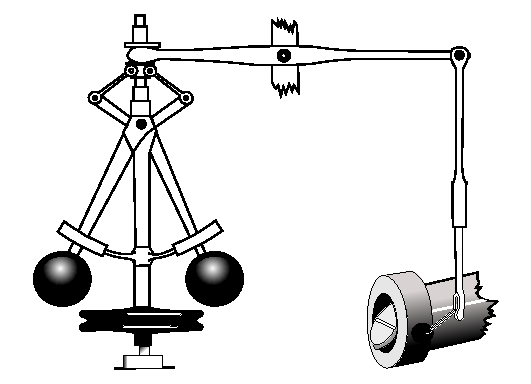
\includegraphics[height=50mm]{Centrifugal_governor.pdf}}

    \figcaption{Wattov regulátor parného stroja, \url{https://en.wikipedia.org/wiki/Centrifugal_governor}}
    \label{Centrifugal_governor}

    }

\end{centering}

Podobné technické riešenia mali veľký vplyv a význam v zmysle industrializácie v~mnohých odvetviach ľudskej činnosti. Neskôr to podnietilo snahy o teoretický rozbor, zovšeobecnenie a matematický opis princípov týchto technických riešení. Intuícia a~invencia pri návrhu takýchto technických riešení viac nepostačovali. Úsilie o~zvýšenie presnosti riadenia viedlo k pomalšiemu tlmeniu kmitania a dokonca až k nestabilite. Nevyhnutnou sa ukazovala potreba vyvinúť teóriu automatického riadenia. V roku 1868 J.~C.~Maxwell formuloval matematickú teóriu súvisiacu s teóriou riadenia, využívajúc diferenciálne rovnice ako model Wattovho regulátora. Maxwellova štúdia sa zaoberala vplyvom rôznych parametrov systému na výslednú kvalitu riadenia. V rovnakom období I.~A.~Vyshnegradskii formuloval matematickú teóriu regulátorov.


Súčasnosť z hľadiska technickej kybernetiky formoval súbeh konkrétnych technických riešení a ich teoretických opisov ako sme ukázali na príklade Wattovho regulátora parného stroja. Historicky ide samozrejme o súčasť priemyselnej revolúcie. Začala v 18. storočí. V podstate pokračuje dodnes a nepochybne bude pokračovať aj v budúcnosti. 



\begin{itemize}[leftmargin=0pt, labelsep=3mm, itemsep=0pt]
    \item 1. priemyselná revolúcia  -- Para \newline Zaradenie parného stroja do výroby. Mechanické riadiace systémy. Neskôr hydraulické a pneumatické.
    \item 2. priemyselná revolúcia  -- Elektrina \newline Zavedenie elektrických zariadení do výroby. Pásová výroba. Optimalizácia procesov. Analógové riadiace systémy.
    \item 3. priemyselná revolúcia  -- Počítače \newline Počítačmi riadená výroba. Číslicové riadiace systémy. Roboty vo výrobe.
    \item 4. priemyselná revolúcia  -- Priemysel 4.0 \newline Inteligentné riadiace systémy a roboty. Presun pracovnej sily z výroby do sféry rozvoja a vývoja. Internet vecí - IoT.
\end{itemize}




% \vbox{
\begin{flushleft}
    \catcode`\-=12


\paragraph{Vybrané historické príklady z oblasti vývoja riadiacich systémov \cite{Bishop2022}}

\setlength\LTleft{0pt}
\setlength\LTright{0pt}

\begin{longtable}{  @{}  l @{\extracolsep{\fill}} p{0.88\textwidth}<{\raggedright} @{}   }



% \begin{tabular*}{\textwidth}{@{}l@{\extracolsep{\fill}}p{0.88\textwidth}<{\raggedright} }
    \toprule
    1788 & Wattov regulátor parného stroja \\ \midrule
    1868 & J. C. Maxwell formuloval matematický model regulácie parného stroja. \\  \midrule
    1913 & Henry Ford zaviedol mechanizovaný montážny stroj na výrobu automobilov. \\  \midrule
    1927 & H. S. Black navrhol zosilňovač so zápornou spätnou väzbou a~H. W. Bode analyzoval spätnoväzbové zosilňovače. \\  \midrule
    1932 & H. Nyquist vyvinul metódu na analýzu stability systémov. \\  \midrule
    1941 & Vznik prvej protilietadlovej zbrane s aktívnym riadením. \\  \midrule
    1952 & Na Massachusetts Institute of Technology bol vyvinutý numerický riadiaci systém (NC) na riadenie osí obrábacích strojov. \\  \midrule
    1954 & George Devol vyvinul „programovaný prenos objektov“ (programmed article transfer),  považovaný za prvý návrh priemyselného robota. \\  \midrule
    1957 & Vypustenie Sputnika odštartovalo vesmírny vek, čo viedlo k miniaturizácii počítačov a~pokroku v~teórii automatického riadenia. \\  \midrule
    1960 & Prvý robot Unimate, založený na Devolových návrhoch, bol predstavený a~v~roku 1961 nainštalovaný na obsluhu strojov pre tlakové liatie. \\  \midrule
    1970 & Vyvinuté modely stavových premenných a~optimálne riadenie. \\ \midrule
    1980 & Robustný návrh riadiacich systémov sa stal predmetom rozsiahleho výskumu. \\  \midrule
    1983 & Zavedenie osobného počítača (a~následného softvéru pre návrh riadenia) prinieslo nástroje na dizajn na stôl inžiniera. \\  \midrule
    1990 & Sieť (vládna) ARPANET (prvá sieť používajúca internetový protokol) ukončila prevádzku a~iné súkromné pripojenia k internetu sa rýchlo rozšírili medzi komerčnými spoločnosťami. \\  \midrule
    1994 & Spätnoväzbové riadenie sa rozšírilo v~automobiloch. Výrobný sektor požadoval spoľahlivé a~robustné systémy. \\  \midrule
    1995 & Globálny systém určovania polohy (GPS) začal poskytovať celosvetové služby pre navigáciu a~synchronizáciu času. \\  \midrule
    1997 & Prvé autonómne rover vozidlo, známe ako Sojourner, skúmalo povrch Marsu. \\  \midrule
    2007 & Misia Orbital Express vykonala prvé autonómne spojenie a~dokovanie vo vesmíre. \\  \midrule
    2011 & NASA Robonaut R2 sa stal prvým robotom z USA na Medzinárodnej vesmírnej stanici, určeným na pomoc pri aktivitách mimo stanice (EVA). \\  \midrule
    2013 & Po prvýkrát sa vozidlo BRAiVE, navrhnuté na Univerzite v~Parme v~Taliansku, pohybovalo autonómne na verejnej ceste bez vodiča na sedadle. \\  \midrule
    2014 & Internet vecí (IoT) bol umožnený rozvojom kľúčových systémov vrátane embedded systémov, bezdrôtových senzorových sietí, riadiacich systémov a~automatizácie. \\  \midrule
    2016 & SpaceX úspešne pristál s prvou raketou na autonómnej plošine, kontrolovanou autonómnym systémom. \\  \midrule
    2019 & Alphabet’s Wing začal prvé komerčné doručovanie dronmi v~USA. \\  
    \bottomrule    
% \end{tabular*}
\end{longtable}


\end{flushleft}
% }










\subsection{Spätná väzba}

Azda najvýznamnejším princípom v Kybernetike je spätná väzba. 

Spätná väzba je významnou črtou života samotného. Spätná väzba ako proces udáva ako rastieme, reagujeme na stres a výzvy a reguluje veličiny ako telesná teplota, krvný tlak a koncentrácia glukózy v krvi. Spätná väzba je prítomná na každej úrovni od vzájomnej interakcie proteínov v bunkách až po interakcie celých organizmov v~komplexných ekologických systémoch \cite{Aastroem2020}.


Spätná väzba je všadeprítomná v prírode. Bez nej by nebola možná evolúcia. Vzorové príklady je možné hľadať predovšetkým v Biológii. Primárne by išlo o príklady tzv. \emph{zápornej spätnej väzby}.

Záporná spätná väzba zabezpečuje reakciu na poruchu alebo narušenie tak aby sa ich efekt znížil. Záporná spätná väzba stabilizuje. Pôsobí proti poruche.

Je možné hovoriť aj o opaku, o \emph{kladnej spätnej väzbe}. 


\paragraph{Príklad kladnej spätnej väzby}

Typickým technickým príkladom kladnej spätnej väzby je situácia, kde máme mikrofón pripojený k reproduktoru. Cez príslušný zosilňovač samozrejme. Zvuk zachytený mikrofónom je reprodukovaný reproduktorom. Ak však mikrofón zachytí zvuk z~reproduktora vznikne tým spätná väzba. Výstup systému sa takpovediac dostane späť na vstup systému. Keďže systém zo vstupu na výstup zosilňuje, tak v tejto situácii mikrofón zachytáva stále silnejší a silnejší zvuk z~reproduktora, ktorý je ďalej a ďalej zosilňovaný. Hovoríme o kladnej spätnej väzbe. Na začiatočný podnet je v systéme kladná odozva, narastajúca odozva, celková zmena výstupu je kladná. Ide samozrejme o neudržateľnú situáciu, o destabilizáciu.

\paragraph{Príklad zápornej spätnej väzby}

Pre príklad zápornej spätnej väzby v systéme je možné uvážiť princíp Wattovho regulátora parného stroja (obrázok \ref{Centrifugal_governor}). Nazýva sa tiež odstredivý regulátor otáčok. Cieľom je regulácie otáčok. Vertikálny hriadeľ je mechanicky spriahnutý zo strojom tak, že jeho otáčky sú proporcionálne otáčkam stroja. Na tomto hriadeli sú zavesené dve závažia. Čí rýchlejšie sa hriadeľ otáča, tým viac sa závažia vzďaľujú od hriadeľa. Zmenu polohy závaží je možné, vhodnou mechanickou konštrukciou, zmeniť na posuvný pohyb ťahadla. Nakoniec týmto pohybom môžeme mechanicky ovládať otvorenie (a~zatvorenie) ventilu pary. Ak sú otáčky stroja nulové, závažia sú v dolnej polohe hneď pri hriadeli, ventil pary je otvorený. Para začne roztáčať hnacie koleso stroja, otáčky sa zvyšujú, poloha závaží sa mení, otvorenie ventilu sa mení -- priviera sa. Postupne sa takto otáčky zvýšia do stavu keď nastane rovnováha v podstate medzi polohou závaží a prívodom pary. Stroj sa neroztočí na vyššie otáčky, pretože závažia by sa viac oddialili od hriadeľa, ventil by sa privrel a menej pary by znamenalo zníženie otáčok. Výstup systému (otáčky) ovplyvňuje vstup systému (prívod pary) tak, že odchýlka od rovnovážneho stavu výstupu spôsobí zmenu vstupu v opačnom zmysle, v negatívnom zmysle, takpovediac so záporným znamienkom. Hovoríme o zápornej spätnej väzbe. 




\subsubsection{Spätná väzba a Teória automatického riadenia}

V kontexte technickej kybernetiky možno vidieť využívanie princípu spätnej väzby ako nástroja pre návrh a syntézu automatických riadiacich systémov, regulačných obvodov a podobne. Pre všeobecný prehľad sa čitateľovi odporúča kniha \emph{Feedback Systems: An~Introduction for Scientists and Engineers} \cite{Aastroem2020}. Do pozornosti sa tiež dáva prehľadový článok \cite{Aastroem2014}.



Teória automatického riadenia je súčasťou kybernetiky. Skúma problematiku zavádzania strojov a~samočinných zariadení s~cieľom riadiť procesy bez priamej účasti človeka. Hoci má využívanie teórie dynamických systémov najväčšie tradície práve v~teórii automatického riadenia, rýchlo nadobúda na význame prakticky vo všetkých disciplínach. Určitou brzdou ich šírenia sú pravdaže vysoké nároky na potrebný matematický aparát, v~prvom rade na riešenie diferenciálnych rovníc. Popri tom však vystupujú aj požiadavky na zručnosti v programovaní a~v~práci s počítačmi \cite{Huba2002}.





\section[Systém, signál, dynamika, stav systému a začiatočné podmienky]{Systém, signál, dynamika,\\ stav systému a začiatočné podmienky}


Teória každého reálneho javu sa zakladá na predstave nazývanej model. Bez zavedenia akýchkoľvek obmedzení model možno reprezentovať matematickými vzťahmi a tieto matematické vzťahy nazývať systém. 

Význam slova systém však chápeme aj širšie. Rôznorodosť reality nie je daná len rôznorodosťou jednotlivých elementov, z ktorých sa skladá. Podstatne viac k~nej prispieva mnohorakosť vzájomného pôsobenia týchto elementov. Intenzita tohto pôsobenia je pritom rôzna: raz intenzívna, inokedy slabá, alebo žiadna.


\paragraph{Systém a signál}

Slovo systém (tiež sústava) používame na označenie určitého počtu elementov, ktorých vzájomné pôsobenie je relatívne intenzívne a možno mu priradiť nejaký význam (zmysel). Interakcie s okolím sú oproti tomu podstatne slabšie.

Súvis systému s okolím vyjadrujeme prostredníctvom väzieb označovaných ako \emph{vstupy a výstupy}.





V kontexte technických súvislostí týmito vstupmi a výstupmi sú veličiny, napríklad teplota, elektrické napätie, výška hladiny a podobne. Tieto sa vo všeobecnosti menia v čase, ich hodnoty sa menia v čase. Súhrnne hovoríme o signáloch, o~vstupných a~výstupných signáloch. Rovnako dobre má význam hovoriť aj o~vstupných a~výstupných veličinách.

Z matematického hľadiska ak hovoríme o signále, tak (takmer vždy) ide o funkciu času. Označme čas $t$. Napríklad výstup systému, výstupnú veličinu systému, označme symbolom $y$. Označenie $y(t)$ znamená, že ide o výstup systému (výstupnú veličinu systému), ktorý je funkciou času $t$. Vo všeobecnosti, mení sa v čase. Hovoríme, že $y(t)$ je signál.

\begin{center}

    \vbox{%
    \makebox[\textwidth][c]{%
	\input{../fig_standalone/schB_signal.pdf_tex}
	}

	\figcaption{Signál v blokovej schéme. Často krát je účelné systémy a signály znázorňovať graficky, schematicky v rámci takzvaných blokových schém. Signál je reprezentovaný čiarou so šípkou, ktorá určuje smer prenosu informácie. Pri čiare je uvedené označenie signálu.}
    \label{schB_signal.pdf}
    }

\end{center}


Pod vstupom systému budeme rozumieť signál, ktorý je vonkajšou príčinou zmien v~systéme. Ak ide o zámerné (želané) zmeny, hovoríme o, všeobecne povedané, riadiacich signáloch, konkrétnejšie v kontexte riadenia systémov hovoríme o akčných zásahoch. Neželané zmeny sú výsledkom pôsobenia vstupných signálov označovaných ako poruchy. 

Má zmysel uvažovať aj systémy, ktoré nemajú definovaný žiadny vstup (napr. generátory signálov). Takéto systémy nazývame aj voľné, autonómne systémy.

Pod výstupom systému zasa rozumieme signál, ktorý v systéme pozorujeme (meriame), alebo signál, ktorým systém pôsobí na svoje okolie. 



\begin{center}

    \vbox{%
    \makebox[\textwidth][c]{%
	\input{../fig_standalone/schB_sys_outonly.pdf_tex}
	}

	\figcaption{Systém s výstupným signálom (s výstupnou veličinou)}
    \label{schB_sys_outonly}
    }

\end{center}

\begin{center}

    \vbox{%
    \makebox[\textwidth][c]{%
	\input{../fig_standalone/schB_sys_SISO.pdf_tex}
	}

	\figcaption{Systém s jedným výstupným signálom a jedným výstupným signálom. SISO systém.}
    \label{schB_sys_SISO}
    }

\end{center}



Systém s jedným vstupom a výstupom nazývame jednorozmerný systém, skrátene SISO systém (z anglického Single Input - Single Output). Znázorňujeme ho blokom (obr. \ref{schB_sys_SISO}). Vstupný signál $u(t)$ a výstupný signál $y(t)$ sú naznačené šípkami.

Systém s viacerymi vstupnými a výstupnými veličinami nazyvame viacrozmerný, alebo MIMO (angl. Multi Input - Multi Output) systém. Vymedzenie vstupných a~výstupných veličín nemusí byť triviálnym a jednoznačným problémom.

\begin{center}

    \vbox{%
    \makebox[\textwidth][c]{%
	\input{../fig_standalone/schB_sys_MIMO.pdf_tex}
	}

	\figcaption{Systém s viacerými vstupnými a výstupnými signálmi. MIMO systém.}
    \label{schB_sys_MIMO}
    }

\end{center}


\paragraph{Dynamický systém}

Napríklad z fyzikálneho hľadiska má často význam zdôrazňovať, že esenciálnou vlastnosťou systému je premenlivosť v čase. O čoho premenlivosť v čase ide môže byť naozaj rôznorodé. Systému dáme prívlastok dynamický.

Prakticky vždy by sme mohli nájsť hľadisko, z ktorého by sme mohli systém označiť za dynamický. Všetko v podstate je dynamický systém. Pri modelovaní a riadení systémov však má veľký význam práve opačné hľadisko, teda rozoznanie systému takého, pri ktorom má zmysel zanedbať jeho prípadné dynamické vlastnosti.

Lepšími pojmami v tejto súvislosti sú \emph{zotrvačnosť a bezzotrvačnosť}.



\subsection{Zotrvačné a bezzotrvačné systémy}


Ak hovoríme o~dynamickom systéme, obvykle máme na mysli \emph{zotrvačný} systém.

\emph{Bezzotrvačný} systém je taký, ktorého výstup závisí len od okamžitej hodnoty vstupu. Minulé hodnoty vstupu nemajú vplyv na aktuálnu hodnotu výstupu. Príkladom bezzotrvačného systému môže byť odporový delič napätia.

O~\emph{zotrvačnom} systéme možno premýšľať ako o~systéme „s pamäťou“. Jeho aktuálny výstup závisí od okamžitej hodnoty vstupu a~aj od hodnôt vstupu v~minulosti. Takýto systém je \emph{kauzálny}.


Mimochodom, teoreticky je možné hovoriť aj o~nekauzálnych systémoch. v~takom prípade výstup závisí aj od budúcich hodnôt vstupu. Slová \emph{zotrvačnosť} a~\emph{kauzalita} tu odporúčame vnímať najmä z fyzikálneho hľadiska.

Príkladom zotrvačného kauzálneho systému môže byť elektrický kondenzátor. Aktuálny elektrický náboj $Q(t)$ na kondenzátore je daný takpovediac celou „históriou“ elektrického prúdu $I(t)$ cez kondenzátor. Formálne, náboj v~čase $t_0$ bude
\begin{equation}
    Q(t_0) = \int_{-\infty}^{t_0}I(t) \text{d}t
\end{equation}



\subsection{Stav systému a začiatočné podmienky}


Predošlá podsekcia navádza na otázky typu ako ďaleko do minulosti ešte ovplyvňujú hodnoty vstupu terajší výstup? Je azda potrebné poznať takpovediac úplnú minulosť systému? Ukazuje sa tu pojem \emph{stav systému}.

Spomínaný náboj $Q$ na kondenzátore má v~čase $t_0$ nejakú hodnotu. Označme ju~$Q_0$. Kondenzátor ako systém je teda v~takom stave, že jeho veličina má hodnotu~$Q_0$. Je to tak presne v~čase $t_0$. 

Ak by sme prišli k tomuto systému v~čase $t_0$, vedeli by sme zistiť, že je v~nejakom stave. v~tomto prípade vyjadriteľnom hodnotou~$Q_0$. Ak by sme chceli zmeniť hodnotu náboja na kondenzátore, teda to v~akom je stave, musíme nejaký čas pôsobiť na vstupe tohto systému (priviesť napätie na svorky kondenzátora).

Poznáme stav systému na začiatku nášho pôsobenia na vstupe a~následne na konci pôsobenia bude vo všeobecnosti systém v~inom stave ako na začiatku. Systém je v~každom čase v~nejakom stave.

Na rozdiel od značne intuitívneho stavu systému v~prípade kondenzátora, určiť ktoré veličiny udávajú stav systému a~či ich vieme merať je samostatná otázka.



\subsubsection{Príklad s mechanickým systémom}


Uvažujme posuvný pohyb telesa s hmotnosťou $m$, na ktoré pôsobí sila $u(t)$. Vo všeobecnosti časovo premenlivá sila je vstupom systému. Teleso sa pohybuje po priamke. Poloha tohto telesa, teda jeho vzdialenosť od stanoveného bodu nula nech je výstupnou veličinou systému. Označme $y(t)$.

\begin{center}

    \vbox{%
        \makebox[\textwidth][c]{%
        \input{../fig_standalone/mechTeleso.pdf_tex}
        }
        \figcaption{Posuvný pohyb telesa s hmotnosťou $m$.}
    }
	\label{mechTeleso}

\end{center}

Pohybová rovnica v~tomto prípade je\footnote{Newtonove $F = ma$ kde $a$ je zrýchlenie, je to druhá derivácia polohy podľa času, teda $\ddot y$.}
\begin{equation} \label{pohybr}
    m \ddot y(t) = u(t)
\end{equation}
Opisuje uvedenú situáciu ako dynamický systém. Dáva do vzťahu vstup a~výstup systému. Je to diferenciálna rovnica druhého rádu.

Ako však určiť v~akom stave je systém? 

Čo potrebujeme poznať, aby sme dokázali určiť výstup systému od nejakého začiatočného času $t_0$ ďalej, teda na intervale $\langle t_0, t \rangle$?

Poloha, výstup systému, je daná začiatočnou polohou v~čase $t_0$, označme $y_0$, a~ďalej je daná integrálom rýchlosti telesa $\dot y(t)$ na uvedenom intervale.
\begin{equation}
    y(t) = y_0 + \int_{t_0}^{t}\dot y(\tau) \text{d}\tau
\end{equation}
kde samozrejme $\tau \in \langle t_0, t \rangle$.

Čím je však potom daný priebeh rýchlosti $\dot y(t)$? Na intervale $\langle t_0, t \rangle$ zjavne musí platiť
\begin{equation}
    \dot y(t) = z_0 + \int_{t_0}^{t}\ddot y(\tau) \text{d}\tau
\end{equation}
kde $z_0$ je začiatočná rýchlosť telesa v~čase $t_0$ a~$\ddot y(t)$ je časový priebeh zrýchlenia telesa. 

Poznáme časový priebeh zrýchlenia na intervale $\langle t_0, t \rangle$? Áno. Priamo vďaka diferenciálnej rovnici opisujúcej samotný systém. Z rovnice \eqref{pohybr} priamo vyplýva
\begin{equation}
    \dot y(t) = \frac{1}{m} \int_{t_0}^{t}  u(\tau) \text{d}\tau
\end{equation}
Časový priebeh vstupného signálu $u(t)$ vo všeobecnosti poznáme. Vstupnú veličinu máme v~moci my.

Na určenie výstupu systému v~čase $t$ sme teda potrebovali poznať nasledovné: začiatočnú polohu, začiatočnú rýchlosť a~časový priebeh vstupnej veličiny od začiatku po čas $t$.

Stav systému na začiatku ale nie len na začiatku je daný dvomi veličinami. Polohou a~rýchlosťou. Ich hodnoty je možné považovať za stav systému. Tieto veličiny možno označiť ako stavové veličiny systému.

Stav systému sa zmení ak nejaký čas bude pôsobiť vstupný signál.



\subsection{Stavový vektor}

Stavových veličín je vo všeobecnosti niekoľko. Minimálne toľko akého rádu je diferenciálna rovnica opisujúca dynamický systém. Hovoríme tak o~ráde systému. V~predchádzajúcom príklade je systém  druhého rádu, $n=2$.

Je praktické usporiadať stavové veličiny do stavového vektora. V~predchádzajúcom príklade sa stavový vektor skladá z dvoch stavových veličín. Stavový vektor označme $x(t)$, formálne sa jeho rozmer uvádza ako $x(t) \in \mathbb R^n$.
\begin{equation}
    x(t) = 
    \begin{bmatrix}
        y(t) \\ \dot y(t)
    \end{bmatrix}
\end{equation}
kde sme uviedli stavové veličiny z predchádzajúceho príkladu. Zvyčajne sa stavové veličiny označujú samostatnými symbolmi, typicky
\begin{equation}
    x(t) = 
    \begin{bmatrix}
        x_1(t) \\ x_2(t)
    \end{bmatrix}
\end{equation}

Prvky stavového vektora $x(t)$ môžu nadobúdať rôzne hodnoty, inými slovami vektor $x(t)$ je v~nejakom priestore, hovoríme o~\emph{stavovom priestore}.










\section{Matematický opis systému}

\subsection{Príklad bezzotrvačného systému}

Uvažujme klasický odporový delič ako je znázornené na nasledujúcom obrázku.


\begin{center}
    \centering

    \makebox[\textwidth][c]{%
    \input{../fig_standalone/OdporovyDelic.pdf_tex}
    }

    \figcaption{Odporový delič}
    \label{OdporovyDelic}
\end{center}

Očividne je tu možné hovoriť o~systéme. Je možné stanoviť výstupný signál a~vstupný signál. Vstupom systému nech je elektrické napätie označené ako $u(t)$ a výstupným signálom nech je napätie $y(t)$.

Nech na vstupe je konštantné napätie, hodnota vstupného signálu $u(t)$  sa nemení, vstup je ustálený. Následkom je, že elektrický prúd cez rezistory $R_1$ a $R_2$ je konštantný, teda $I(t) = u(t) / (R_1 + R_2)$. Napätie na rezistore $R_2$ je potom $y(t) = R_2 I(t) = R_2 u(t) / (R_1 + R_2)$. Vzťah medzi výstupom a vstupom systému opisuje rovnica
\begin{equation} \label{odporovydelic}
    y(t) = \frac{R_2}{R_1 + R_2} u(t)
\end{equation}
Táto rovnica je matematickým modelom systému.

Ak by sme na vstupe uvažovali časovo premenlivý signál $u(t)$, tak táto rovnica by stále platila. Stále by bola užitočnou z hľadiska matematického modelovania systému. 

Rovnica \eqref{odporovydelic} je algebraická rovnica. Nie je to diferenciálna rovnica. Neznámou v~rovnici je výstupný signál $y(t)$ a v rovnici nevystupuje derivácia neznámej. V~takomto prípade hovoríme o bezzotrvačnom systéme. V~tomto prípade nie je účelné uvažovať o systéme ako o dynamickom. V~okamihu ako je daná hodnota $u(t)$, v~tom istom okamihu je daná hodnota $y(t)$. Niekedy hovoríme o takomto systéme ako o statickom v zmysle, že nemá zmysel uvažovať dynamiku systému a tak systém je statický.

\subsubsection{Zosilnenie systému}

O ustálenom stave systému, teda situácií keď vstup $u(t)$ a výstup $y(t)$ nemenia svoju hodnotu, je však dôležité uvažovať vždy. O ustálenom stave je možné uvažovať ako o~vlastnosti systému. Buď je možné, aby bol systém v ustálenom stave alebo to možné nie je.

Ak je možné, aby bol systém v ustálenom stave, hovoríme, že systém je statický. Ak to nie je možné, hovoríme o astatickom systéme, teda takom, pri ktorom aj keď vstup je ustálený, výstup sa nikdy neustáli.

Hodnoty vstupu a výstupu v ustálenom stave sa označujú napríklad ako $y(\infty)$ a~$u(\infty)$, kde $\infty$ značí čas „v nekonečne“, čo v praxi je taký čas, ktorý je potrebný pre praktické ustálenie sa hodnôt daných signálov.

Ak je možné aby bol systém v ustálenom stave, tak túto vlastnosť vystihuje pojem \emph{statické zosilnenie systému} prípadne len \emph{zosilnenie systému}. Zosilnenie systému je pomer medzi ustálenou hodnotou výstupného signálu systému a~ustálenou hodnotou vstupného signálu systému. Označme ho $K$. Teda
\begin{equation}
    K = \frac{y(\infty)}{u(\infty)}
\end{equation}





\subsection{Príklad dynamického systému}

Majme RC obvod ako je znázornené na obr.~\ref{RCobvod}. Nech je na začiatku, v čase $t=0$, kondenzátor $C$ nabitý a na jeho svorkách je napätie s~hodnotou $u_0$. Inými slovami napätie $u(t)$ v čase $0$ je $u_0$, teda $u(0) = u_0$. Ku kondenzátoru $C$ je pripojený rezistor $R$ a preto sa kondenzátor s rastúcim časom vybíja.

\begin{center}

	\makebox[\textwidth][c]{%
	\input{../fig_standalone/RCobvod.pdf_tex}
	}

	\figcaption{RC obvod}
	\label{RCobvod}
\end{center}

Ide o systém, ktorý má len výstupný signál. Výstupom je napätie na kondenzátore $C$, v tomto prípade označené ako $u(t)$. Z~fyzikálnej podstaty veci je možné napätie na kondenzátore opísať diferenciálnou rovnicou v tvare
\begin{equation} \label{diffR}
    \dot Q(t) = - \frac{1}{RC} Q(t)
\end{equation}
pričom $Q(t)$ je elektrický náboj na kondenzátore a pre samotné napätie na kondenzátore platí $u(t) = Q(t) / C$.

Matematickým modelom systému je teda diferenciálna rovnica. Neznámou v rovnici v tomto prípade je $Q(t)$. Ak poznáme $Q(t)$, poznáme tým aj výstup systému.

Keďže matematickým opisom systému je diferenciálna rovnica, teda v rovnici figurujú aj derivácie neznámej, tak hovoríme o dynamickom systéme. Inými slovami o zotrvačnom systéme, v tomto prípade je zotrvačnosť zrejmá z podstaty kondenzátora, ktorý nie je možné vybiť okamžite.

Neznámou diferenciálnej rovnice je funkcia, v tomto prípade funkcia času. Neznáma diferenciálnej rovnice teda zodpovedá signálu systému, principiálne výstupu systému. Vlastnosti systému, jeho dynamiku, tak môžme skúmať tak, že nájdeme riešenie diferenciálnej rovnice.


\subsubsection{Riešenie diferenciálnej rovnice}

Zaoberáme sa diferenciálnou rovnicou v tvare
\begin{equation} \label{diffRbeta}
    \frac{\text{d}Q(t)}{\text{d}t} = - \frac{1}{RC} Q(t) \qquad Q(0) = Q_0
\end{equation}
kde $Q(t)$ je neznáma časová funkcia. Nezávisle premennou v tejto funkcii je čas $t$, závisle premennou je „$Q$“.  Konštanty (nie sú funkciou času) $R$, $C$ a aj $Q_0$ sú známe. 

Upravme diferenciálnu rovnicu \eqref{diffRbeta} tak, aby rovnaké premenné ($Q(t)$ a $t$) boli na rovnakých stranách. V tvare \eqref{diffRbeta} je signál $Q(t)$ na oboch stranách rovnice. Nech je len na ľavej strane. Rovnako, nech čas $t$ je len na pravej strane. Teda
\begin{equation} \label{diffRbeta2}
    \frac{1}{Q(t)}\text{d}Q(t) = - \frac{1}{RC} \text{d}t
\end{equation}

Všimnime si, že teraz je možné obe strany rovnice integrovať, každú podľa vlastnej premennej, teda
\begin{equation} \label{diffRbeta3}
    \int \frac{1}{Q(t)}\text{d}Q(t) =  \int - \frac{1}{RC} \text{d}t
\end{equation}
Výsedkom inegrovania je
\begin{equation} \label{diffRbeta4}
     \ln \left(  Q(t)  \right) + k_1 =   - \frac{1}{RC} t + k_2
\end{equation}
kde $k_1$ a $k_2$ sú konštanty vyplývajúce z neurčitých integrálov (a tiež $Q(t)>0 \ \forall \ t$).

Rovnica \eqref{diffRbeta4} už nie je diferenciálna. Žiadna veličina v nej nie je derivovaná podľa času. Vyjadrime z rovnice \eqref{diffRbeta4} signál $Q(t)$. Úpravou
\begin{align}
    \ln \left(  Q(t)  \right)  =   - \frac{1}{RC} t + k_3
\end{align}
sme zaviedli konštantu $k_3 = k_2 - k_1$. Ďalej
\begin{subequations}
    \begin{align}
        Q(t)   &=  e^{\left( - \frac{1}{RC} t + k_3 \right)} \\
        Q(t)   &=  e^{\left( - \frac{1}{RC} t \right)}  e^{k_3} \label{rawRies}
    \end{align}
\end{subequations}
Je možné ukázať, že platí $e^{k_3} = Q_0$.

Hľadaným riešením diferenciálnej rovnice je časová funkcia v tvare
\begin{align}
    Q(t)   &=  Q_0 \ e^{\left( - \frac{1}{RC} t \right)}   \label{rawRies2}
\end{align}









\section[Schematické znázornenie dynamického systému]{Schematické znázornenie dynamického systému\\ (diferenciálnej rovnice)}


Majme diferenciálnu rovnicu v tvare:
\begin{equation} \label{hodrpr01}
    \frac{\text{d}y(t)}{\text{d}t} = - a y(t) \qquad y(0)=y_0
\end{equation}
kde $y(t)$ je neznáma funkcia času, riešením rovnice hľadáme túto funkciu času, a $a\in\mathbb{R}$ (je to reálne číslo) je daný parameter. Hodnota $y_0$ v začiatočnej podmienke je tiež daná.

\subparagraph{Poznámka:} Všimnime si, že rovnice \eqref{hodrpr01} a \eqref{diffRbeta} sú v podstate rovnaké. V~rovnici \eqref{diffRbeta} je $a = 1/(RC)$ a $y(t)$ je v~rovnici \eqref{hodrpr01} to isté ako $Q(t)$ v~rovnici \eqref{diffRbeta}.

Ak by sme členy obsahujúce len neznámu $y(t)$ presunuli na ľavú stranu, teda:
\begin{equation}
    \frac{\text{d}y(t)}{\text{d}t} + a y(t) = 0
\end{equation}
na pravej strane je nula. Hovoríme, že rovnica je homogénna.

Deriváciu funkcie $y(t)$ podľa času, teda $\frac{\text{d}y(t)}{\text{d}t}$ je praktické označovať aj ako $\dot y(t)$. V~takomto prípade je rovnica \eqref{hodrpr01} v tvare
\begin{equation} \label{eq:HDR1R}
    \dot y(t) + a y(t) = 0 
\end{equation}
alebo 
\begin{equation} \label{eq:HDR1Rs}
    \dot y(t) = - a y(t)
\end{equation}

Ak táto rovnica opisuje dynamický systém, tak je zrejmé, že existuje signál $\dot y(t)$. Inými slovami, to, čo určite máme k dispozícii je signál $\dot y(t)$. Ak by tento signál neexistoval, tak vlastne rovnica \eqref{eq:HDR1Rs} by bola nezmyslom. Schematicky teda môžeme vyjadriť, že teda máme k~dispozícii signál $\dot y(t)$.
\begin{center}

    \vbox{%
    \makebox[\textwidth][c]{%
    \input{../fig_standalone/schB_pr0_k1.pdf_tex}
    }

    \vspace{-5mm}

    \figcaption{Bloková schéma rovnice \eqref{eq:HDR1R}, krok prvý.}
    \label{schB_pr0_k1.pdf}
    }

\end{center}
Rovnica v tvare \eqref{eq:HDR1Rs} tiež priamo ukazuje, že signál $\dot y(t)$ je to isté ako výraz $- a y(t)$. Vieme zostaviť blokovú schému tohto výrazu? Ide zjavne o zosilňovač so zosilnením $-a$, ktorý má na vstupe signál $y(t)$. Pridajme do blokovej schémy:
\begin{center}

    \vbox{%
    \makebox[\textwidth][c]{%
    \input{../fig_standalone/schB_pr0_k2.pdf_tex}
    }

    \figcaption{Bloková schéma rovnice \eqref{eq:HDR1R}, krok druhý.}
    \label{schB_pr0_k2.pdf}
    }

\end{center}
Keďže doslova $\dot y(t) = - a y(t)$, tak
\begin{center}

    \vbox{%
    \makebox[\textwidth][c]{%
    \input{../fig_standalone/schB_pr0_k3.pdf_tex}
    }

    \figcaption{Bloková schéma rovnice \eqref{eq:HDR1R}, krok tretí.}
    \label{schB_pr0_k3.pdf}
    }

\end{center}
Pripomeňme, že signál $\dot y(t)$ takpovediac existuje, je k dispozícii. Samotný signál $y(t)$ však nie je k dispozícii. Je potrebné ho vytvoriť z toho, čo už k dispozícii je. Je zrejmé, že signál $y(t)$ je možné získať integrovaním $\dot y(t)$, teda
\begin{center}

    \vbox{%
    \makebox[\textwidth][c]{%
    \input{../fig_standalone/schB_pr0_k4.pdf_tex}
    }

    \figcaption{Bloková schéma rovnice \eqref{eq:HDR1R}, krok štvrtý.}
    \label{schB_pr0_k4.pdf}
    }

\end{center}
pričom integrátor musí mať začiatočnú podmienku $y(0) = y_0$ (podľa \eqref{eq:HDR1R}).
\begin{center}

    \vbox{%
    \makebox[\textwidth][c]{%
    \input{../fig_standalone/schB_pr0_k4b.pdf_tex}
    }

    \figcaption{}
    \label{schB_pr0_k4b.pdf}
    }

\end{center}
Napokon
\begin{center}

    \vbox{%
    \makebox[\textwidth][c]{%
    \input{../fig_standalone/schB_pr0_k5.pdf_tex}
    }

    \figcaption{Bloková schéma rovnice \eqref{eq:HDR1R}.}
    \label{schB_pr0_k5.pdf}
    }

\end{center}
je bloková schéma dynamického systému, ktorá zodpovedá diferenciálnej rovnici \eqref{eq:HDR1R}.









\printbibliography[title={Literatúra}]





\end{document}
